\documentclass[a4paper,12pt]{book}
\usepackage[utf8]{inputenc}

\usepackage{rachwidgets}


\newcommand{\laClass}       {CS 210}
\newcommand{\laSemester}    {Spring 2018}
\newcommand{\laChapter}     {1.1}
\newcommand{\laType}        {Exercise}
\newcommand{\laPoints}      {5}
\newcommand{\laTitle}       {First Examples}
\newcommand{\laDate}        {Week 1}
\setcounter{chapter}{5}
\setcounter{section}{1}
\addtocounter{section}{-1}
\newcounter{question}

\toggletrue{answerkey}
\togglefalse{answerkey}


\title{}
\author{Rachel Singh}
\date{\today}

\pagestyle{fancy}
\fancyhf{}

\lhead{\laClass, \laSemester, \laDate}

\chead{}

\rhead{\laChapter\ \laType\ \iftoggle{answerkey}{ KEY }{}}

\rfoot{\thepage\ of \pageref{LastPage}}

\lfoot{\scriptsize By Rachel Singh, last updated \today}

\renewcommand{\headrulewidth}{2pt}
\renewcommand{\footrulewidth}{1pt}

\begin{document}




\notonkey{

\footnotesize
~\\ 
\textbf{\laChapter\ \laType: } In-class exercises are meant to introduce you to a new topic
and provide some practice with the new topic. Work in a team of up to 4 people to complete this exercise.
You can work simultaneously on the problems, or work separate and then check your answers with each other.
You can take the exercise home, score will be based on the in-class quiz the following class period.
\textbf{Work out problems on your own paper} - this document just has examples and questions.

\hrulefill
\normalsize 

}{
\begin{center}
    \Large
    \textbf{Answer Key}
\end{center}
}


\notonkey{
    \section{\laTitle}

    \subsection{Coin Toss}

    \begin{intro}{Coin toss}
        When we're flipping a coin, there are two possible outcomes:
        \textit{heads} or \textit{tails}. If we flip more than one
        coin, then we end up with more possible outcomes. For example,
        when flipping two coins, we have four possible outcomes:

        \begin{center}
            \begin{tabular}{ | l | c | c | }
                \hline
                1. & HEADS & HEADS \\ \hline
                2. & HEADS & TAILS \\ \hline
                3. & TAILS & HEADS \\ \hline
                4. & TAILS & TAILS \\ \hline
            \end{tabular}
        \end{center}
    \end{intro}

    % - QUESTION --------------------------------------------------%
    \stepcounter{question}
    \begin{questionNOGRADE}{\thequestion}
        Draw a table of all possible outcomes if someone flips three coins.
    \end{questionNOGRADE}

    % - QUESTION --------------------------------------------------%
    \stepcounter{question}
    \begin{questionNOGRADE}{\thequestion}
        Write out how many outcomes there are for each of the following.

        \begin{tabular}{p{6cm} p{6cm}}
            a. Flipping one coin &
            b. Flipping two coins \\
            c. Flipping three coins &
            d. Rolling one 6-sided die \\
            e. Rolling two 6-sided dice &
            f. Rolling three 6-sided dice
        \end{tabular}
    \end{questionNOGRADE}

    % - QUESTION --------------------------------------------------%
    \stepcounter{question}
    \begin{questionNOGRADE}{\thequestion}
        Using the variables \texttt{outcomesPerEvent},
        \texttt{eventExecutions}, and \texttt{totalOutcomes},
        write an equation (line of code) that uses \texttt{outcomesPerEvent}
        and \texttt{eventExecutions} to find the value of \texttt{totalOutcomes}.
        Use $\wedge$
        to represent exponent.

        \texttt{totalOutcomes = }
    \end{questionNOGRADE}

    \newpage

    \subsection{Josephus game}

    \begin{intro}{The Josephus game}
        The Josephus game is a theoretical problem, and for now we
        will just solve it systematically by stepping through the
        instructions given.

        \paragraph{Setup:} People are sitting in a circle, each with
        an assigned number (their location in the circle).

        \paragraph{Step:} People are eliminated at every $n$th step,
        with counting beginning at the $n$th person.

        \paragraph{Result:} After stepping through, figure out the
        position of the \textit{last} and \textit{second-to-last}
        person left (not eliminated).

        \paragraph{Example:} Let's say that we begin with a circle of
        \textit{10} people, numbered from 1 to 10. We will eliminate
        people at an interval of \textit{2} - so, every-other-person,
        beginning with person \#2. Who will be the last person standing?

        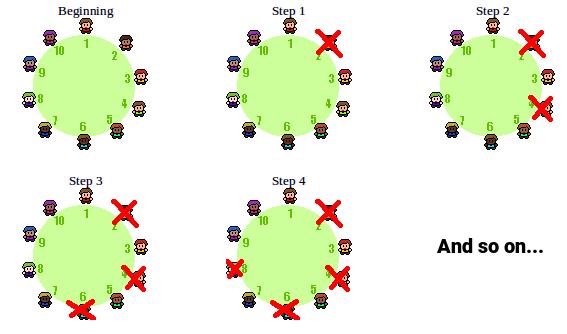
\includegraphics[width=12cm]{images/josephus.png}
    \end{intro}

    \newpage

    % - QUESTION --------------------------------------------------%
    \stepcounter{question}
    \begin{questionNOGRADE}{\thequestion}
        Given a Josephus circle of 15 people,
        if we are eliminating every 3rd person (starting with person 3),
        who is the last to be ``killed" – and the 2nd to last to be ``killed"?

        \begin{center}
            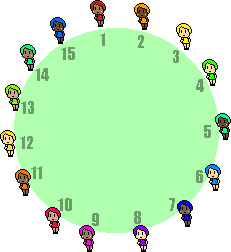
\includegraphics[width=6cm]{images/josephus-15.png}
        \end{center}

        \begin{hint}{Hint:}
            Don't count ``dead" people, make sure to skip over them!
        \end{hint}
        
    \end{questionNOGRADE}

    % - QUESTION --------------------------------------------------%
    \stepcounter{question}
    \begin{questionNOGRADE}{\thequestion}
        Given a Josephus circle of 10 people,
        if we are eliminating every 4th person (starting with person 4),
        who is the last to be ``killed" – and the 2nd to last to be ``killed"?

        \begin{center}
            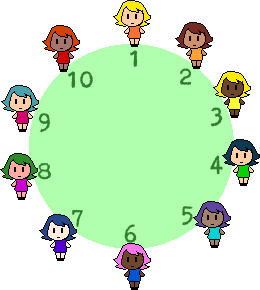
\includegraphics[width=7cm]{images/josephus-10.png}
        \end{center}
    \end{questionNOGRADE}
    
    \subsection{Game trees}

    \begin{intro}{Game trees}
        In section 1.1, we will also be looking at events that have multiple outcomes –
        such as flipping one coin, two coins, or three coins, or who of two people win
        one, two, or three tennis matches. With small amounts of ``variables", we can
        list out all the possible outcomes, and we can build a game tree based on this.
        
        \paragraph{Example:} ~\\
        If you flip one coin, the result with be HEADS (H) or TAILS (T).
        If you flip two coins, what are all the outcomes?

        \begin{center}
            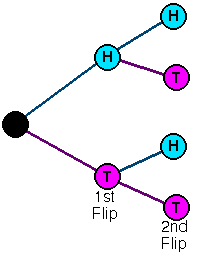
\includegraphics[width=5cm]{images/gametree.png}
            
            \begin{tabular}{l l}
                1. HH &  2. HT \\
                3. TH &  4. TT
            \end{tabular}
        \end{center}

    \end{intro}

    % - QUESTION --------------------------------------------------%
    \stepcounter{question}
    \begin{questionNOGRADE}{\thequestion}
        Suppose you toss three coins – a nickel, a dime, and a quarter,
        and you record the results in that order. For example,
        ``HTH" means nickel = heads, dime = tails, quarter = heads.

        \begin{enumerate}
            \item[a.] In a systematic way, list all the different results you could record.
            \item[b.] Draw a game tree for recording the results.
            \item[c.] On the game tree, label each possible result either 0, 1, 2, or 3,
            to indicate how many \textit{heads} there are.
            \item[d.] Do you think a person who tosses three coins is more likely to get all
            three heads, or to get exactly two heads?                
        \end{enumerate}
    \end{questionNOGRADE}
    
    
}{
    \begin{enumerate}
        \item[1.]   
                \begin{tabular}{ | l | c | c | c | }
                    \hline
                    1. & HEADS & HEADS & HEADS \\ \hline
                    2. & HEADS & HEADS & tails \\ \hline
                    3. & HEADS & tails & HEADS \\ \hline
                    4. & HEADS & tails & tails \\ \hline
                    5. & tails & HEADS & HEADS \\ \hline
                    6. & tails & HEADS & tails \\ \hline
                    7. & tails & tails & HEADS \\ \hline
                    8. & tails & tails & tails \\ \hline
                \end{tabular}

        \item[2a.]  $2^{1} = 2$
        \item[2b.]  $2^{2} = 4$
        \item[2c.]  $2^{3} = 8$
        \item[2d.]  $6^{1} = 6$
        \item[2e.]  $6^{2} = 36$
        \item[2f.]  $6^{3} = 216$

        \item[3.]   \texttt{totalOutcomes = outcomesPerEvent $\wedge$ eventExecutions}

        \item[4.]   2nd-to-last: Person 14; last: Person 5

        \item[5.]   2nd-to-last: Person 6; last: Person 5

        \item[6a.]   1. HHH, 2. HHT, 3. HTH, 4. HTT, \\ 5. THH, 6. THT, 7. TTH, 8. TTT
        \item[6b.]  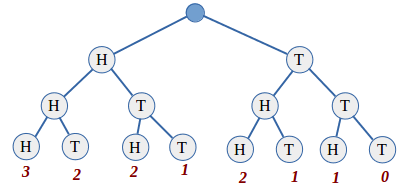
\includegraphics[width=6cm]{images/ans-gametree.png}
        \item[6c.]  ...
        \item[6d.]  More likely to get exactly 2 heads.
    \end{enumerate}
}

    



\end{document}

